\documentclass[xcolor={rgb}]{beamer}
\usepackage[labelformat=empty]{caption}
\usepackage[outputdir=out]{minted}
\usepackage{metalogo}
\usepackage{fontspec}
\usepackage{tikz}

\newcommand{\pitem}{\pause \item}
\usetheme{Arguelles}

\newcommand{\img}[3]{
  \only<#1>{
    \begin{figure}
      \includegraphics[width=\textwidth]{#2}
      \caption{#3}
    \end{figure}
  }
}

\newcounter{_i}
\newcommand{\starcounting}{\setcounter{_i}{2}}
\newcommand{\simg}[2]{
  \stepcounter{_i}
  \img{\value{_i}}{#1}{#2}
}

\author{Alireza Arzehgar}
\title{Introduction to \\{\color{red}Remote Procedure Call (RPC)}}
\date{\today}

\begin{document}
\begin{frame}[plain]
  \titlepage
\end{frame}


\begin{frame}{The simplest possible explanation}
  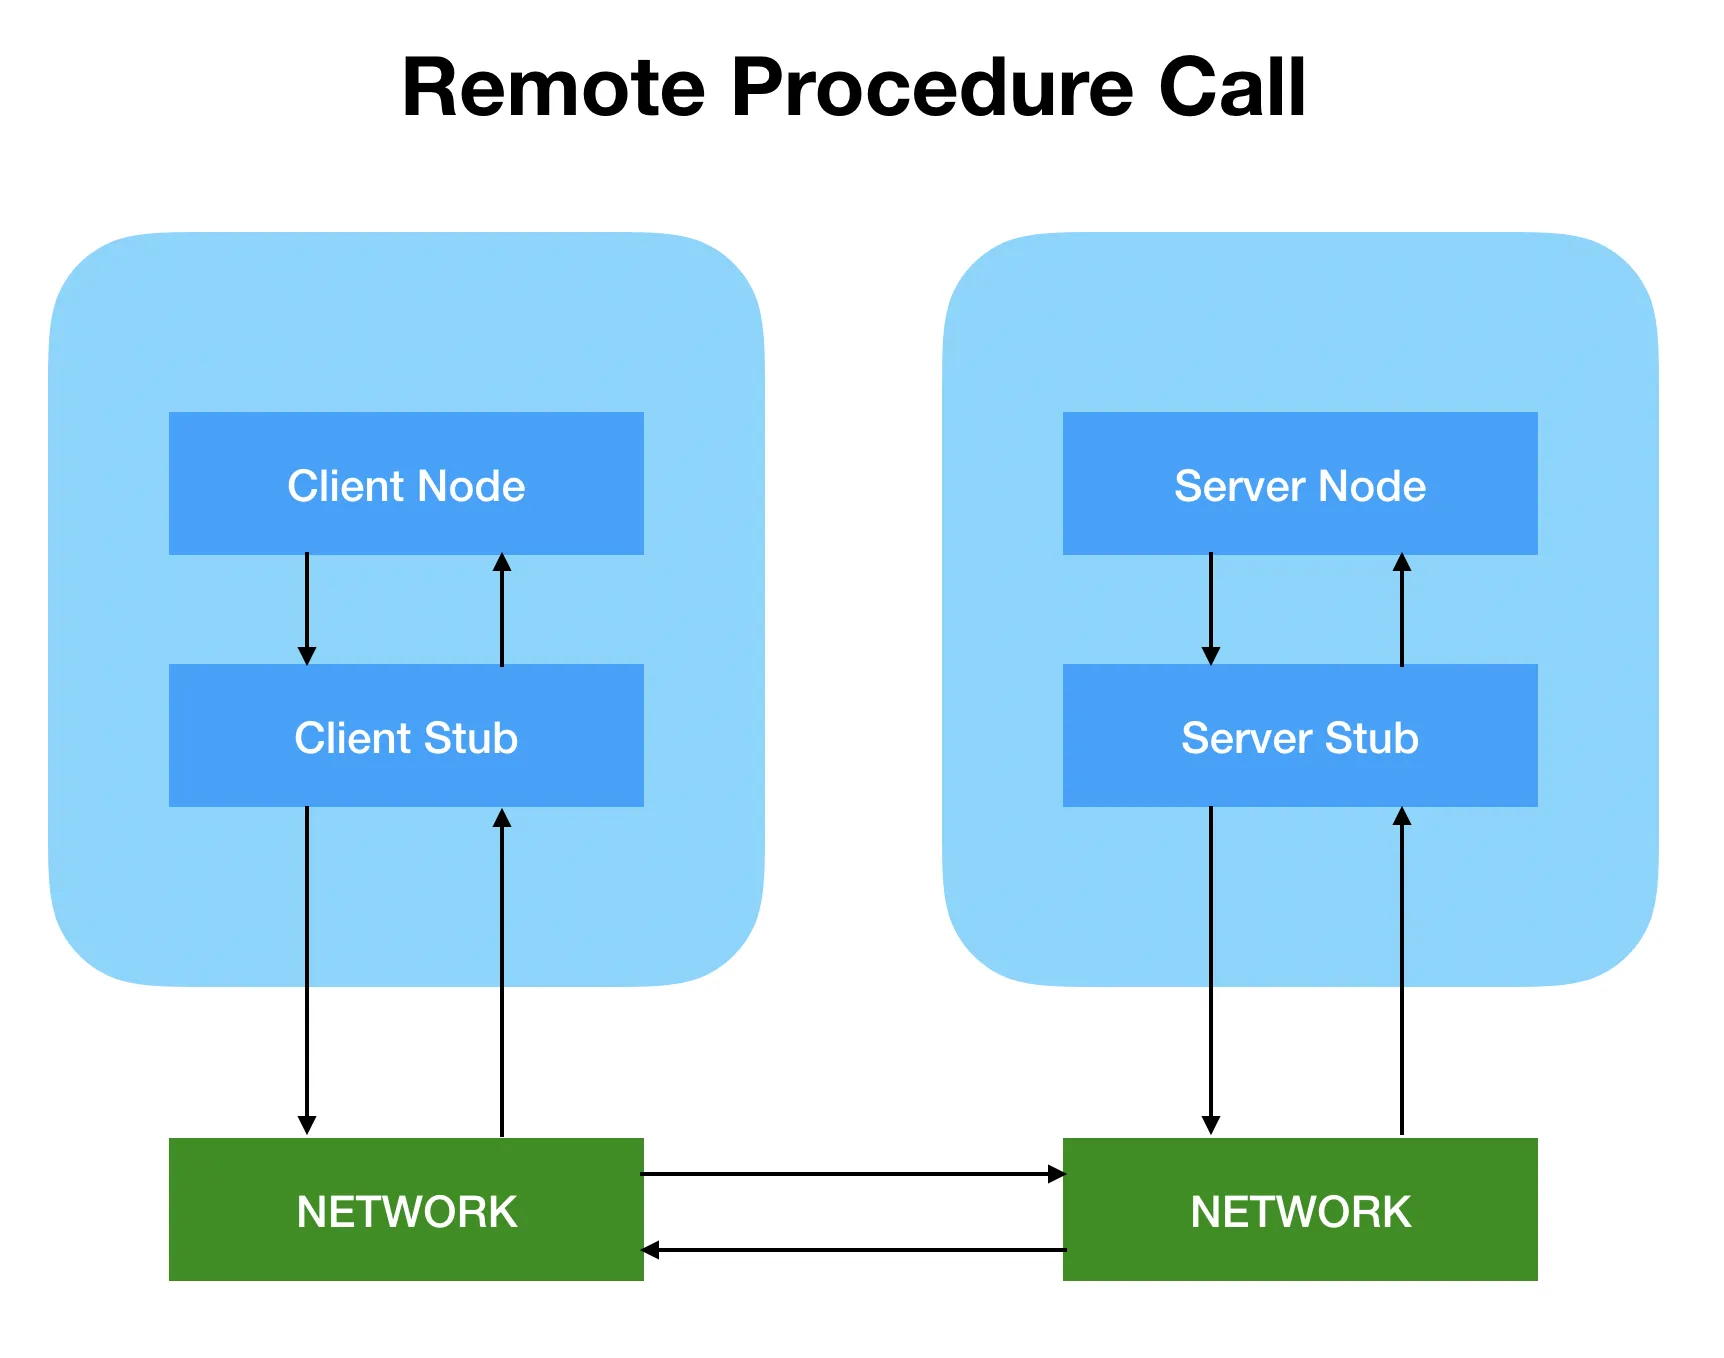
\includegraphics[width=\textwidth]{assets/RPC.png}
\end{frame}

\begin{frame}{What is Remote Procedure Call?}
  % A person who shouted to other with a call

  {\Large Definitions:}
  \begin{itemize}
      \pitem A way to execute a \textbf{procedure} that could be running in a separate application on the same
      machine or even potentially on the network. (\textit{Building Microservices with Go})
      \pitem A client-server mechanism for \textbf{interprocess communication}. (\textit{Mastering Go second edition})
  \end{itemize}

  \vspace{0.3cm}

  \pause
  {\Large Implementation Stages:}
  \begin{itemize}
      \pitem Design a interface definition.
      \pitem Develop server-side application.
      \pitem Architect client-side program.
  \end{itemize}
\end{frame}

\begin{frame}[fragile]{Simple Golang RPC Interface Definition}
  \begin{minted}{go}
type HelloService interface {
  Print(*Request, *Response) error
}

type Request struct{}

type Response struct {
  Msg string
}
  \end{minted}
\end{frame}

\begin{frame}[fragile]{Simple Golang RPC Client}
  \begin{minted}{go}
// client.go
func main() {
  c, _ := rpc.Dial("tcp", "localhost:8000")

  var reply Response
  c.Call("Hello.Print", &Request{}, &reply)

  fmt.Println(reply.Msg)
}

// OUTPUT: Hello, World!
  \end{minted}
\end{frame}

\begin{frame}[fragile]{Simple Golang RPC Server}
  \begin{minted}{go}
// server.go
type Hello struct{}

func (Hello) Print(req *Request, res *Response) error {
  res.Msg = "Hello, World!"
  return nil
}

func main() {
  rpc.Register(new(Hello))
  l, _ := net.Listen("tcp", ":8000")
  for {
    conn, _ := l.Accept()
    rpc.ServeConn(conn)
  }
}
  \end{minted}
\end{frame}

\begin{frame}{History}
  \begin{itemize}
    \pitem Sun's RPC (ONC RPC) - \textit{1981}
    \pitem Remote Method Invocation (RMI) - \textit{1990}
    \pitem HTTP 1 - \textit{1996}
    \pitem REST - \textit{2000}
    \pitem Apache Thrift - \textit{2007}
    \pitem HTTP 2 - \textit{2015}
    \pitem gRPC - \textit{2015}
  \end{itemize}
\end{frame}

\begin{frame}{The Advantages of gRPC}
  \begin{itemize}
    \pitem Code generators
    \pitem Speed and performance
    \pitem Type safety
    \pitem Self documented architecture
    \pitem Support streaming, authentication, load balancing, etc.
  \end{itemize}
\end{frame}

\begin{frame}[fragile]{Protocol Buffer (protobuf) Example}
  \begin{minted}{proto}
// api.proto
syntax = "proto3";
option go_package = "/main";

service Hello {
  rpc Print (Request) returns (Response);
}

message Request {}

message Response {
  string Message = 1;
}
  \end{minted}

  \pause

  \vspace{-0.5cm}
  \noindent\rule{\textwidth}{0.1pt}
  \begin{minted}[fontsize=\footnotesize]{bash}
$ protoc --go_out=. --go_opt=module=/main \
  --go-grpc_opt=paths=source_relative \
  --go-grpc_out=.  ./api.proto
  \end{minted}
\end{frame}

\begin{frame}[fragile]{gRPC Client}
  \begin{minted}{go}
// client.go
func main() {
  remote := "localhost:8000"
  conn, _ := grpc.Dial(remote, grpc.WithInsecure())
  client := NewHelloClient(conn)
  r, _ := client.Print(context.Background(), &Request{})

  fmt.Println(r.Message)
}

// OUTPUT: Hello, World!
  \end{minted}
\end{frame}

\begin{frame}[fragile]{gRPC Server}
  \begin{minted}[fontsize=\footnotesize]{go}
// server.go
type hello struct {
  UnimplementedHelloServer
}

func (hello) Print(c context.Context, r *Request) (*Response, error) {
  return &Response{Message: "Hello, Wrold"}, nil
}

func main() {
  s := grpc.NewServer()
  RegisterHelloServer(s, hello{})

  l, _ := net.Listen("tcp", ":8000")
  s.Serve(l)
}
  \end{minted}
\end{frame}

\begin{frame}[fragile]{Where You Should Embrace RPC}
  \begin{itemize}
    \pitem Communication between microservices
    \pitem Performance critical projects
    \pitem Work with blockchain technologies (JSON-RPC)
    \pitem Components are tightly coupled
  \end{itemize}
\end{frame}

\begin{frame}
  \vfill
  \begin{center}
    \Huge Tell us about your experiences
  \end{center}
  \vfill
\end{frame}
\end{document}
